\section[轨迹]{轨~~~~迹}\label{sec:01.05}

谁都看到过,当喷气式飞机在飞行的时候,它的尾部泄出的
白烟在天空中构成形状美丽的各样曲线。这些曲线反映了飞机所
行经的路程。质点在运动中所经过的各点在空间连成一条曲线,
这条曲线我们称之为轨迹。

\begin{figure}[!h]
    \hspace{3em}
    \subfigure[\null]{
        \label{fig:01.06a}
        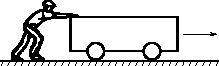
\includegraphics{figure/fig01.06a}
    }
    \hspace{3em}
    \subfigure[\null]{
        \label{fig:01.06b}
        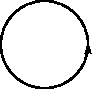
\includegraphics{figure/fig01.06b}
    }

    \hspace{3.7em}
    \subfigure[\null]{
        \label{fig:01.06c}
        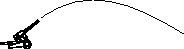
\includegraphics{figure/fig01.06c}
    }
    \hspace{1.3em}
    \subfigure[\null]{
        \label{fig:01.06d}
        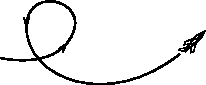
\includegraphics{figure/fig01.06d}
    }
    \caption{各种运动的轨迹}
    \label{fig:01.06}
\end{figure}

\clearpage

从图\ref{fig:01.06}~看到,各种运动的轨迹形状是不同的;\subref{fig:01.06a}图是直线,
\subref{fig:01.06b}图是圆周,\subref{fig:01.06c}图是抛物线,\subref{fig:01.06d}图是一般曲线。依照轨迹形状
的不同,可以把运动分为直线运动和曲线运动两大类。

如何描写轨迹呢?可利用曲线方程来描写。譬如,曲线方程 \begin{equation*}
    \begin{aligned}
        &x^2+y^2=r^2 \\[-0.5em]
        &z=0
   \end{aligned}
\end{equation*}
就描写了在$z=0$平面上半径为$r$的圆周运动的轨迹。一般曲线方
程可以表示成
\begin{equation*}
    \begin{aligned}
        f_1(x,y,z)=0 \\[-0.5em]
        f_2(x,y,z)=0
    \end{aligned}
\end{equation*}

在历史上很长一个时期内,人们只注重轨迹形状的研究,例
如行星走圆形,落体走直线。我们知道,质点运动是位置的变化,
它涉及空间和时间两方面。轨迹形状只反映了运动的空间方面的
性质,它对于研究运动还是不够的,因为轨迹还没有把质点运动
的情况全部表述出来,特别是没有表述它的动态性质。百米赛跑
时,所有运动员的轨迹都是直线,但他们各自的运动情况并不全
同,否则就分不出名次了。我们不仅应该知道轨迹,而且还应知
道质点经过轨迹上各点的时刻。运动是在时间、空间里的现象,
关键是把时间描写和空间描写联系起来。直到牛顿之前不久,才
特别强调了这一点。

下面,我们举两个直线运动的例子。

对于在平直铁轨上稳定运动的列车上的某一点,所测得的各
时刻的位置列于表\ref{tab:01.04}~中,其中位置坐标$x$是以铁轨为参考系的(图\ref{fig:01.07})。
\vspace{-1em}
\begin{tablex}[!h]
    \caption{}
    \label{tab:01.04}
    \centering
        \begin{tabularx}{\linewidth}{c*{6}{|C}}
            \toprule
            时~~~~间(秒) & 0 & 1  & 2  & 3  & 4  & 5  \\
            \midrule
            位置坐标(米) & 0 & 17 & 34 & 51 & 68 & 85 \\
            \bottomrule
        \end{tabularx}
\end{tablex}

\begin{figurex}[!h]
    \centering
    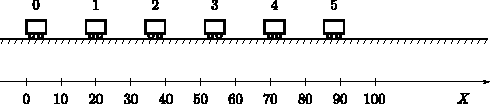
\includegraphics{figure/fig01.07}
    \caption{列车的运动}
    \label{fig:01.07}
\end{figurex}

对于从地面上某一高度自由落下的质点(称为自由落体),轨
迹也是一条直线。如果我们取如图\ref{fig:01.08}~所示的坐标系,则所测得的
质点在各时刻的位置列在表\ref{tab:01.05}~中。
\begin{tablex}[!h]
    \caption{}
    \label{tab:01.05}
    \centering
        \begin{tabularx}{\linewidth}{c*{5}{|C}}
            \toprule
            时~~~~间(秒) & 0 & 1   & 2    & 3    & 4    \\
            \midrule
            位置坐标(米) & 0 & 4.9 & 19.6 & 44.1 & 78.4 \\
            \bottomrule
        \end{tabularx}
\end{tablex}

用数学的语言说,表\ref{tab:01.04}~和表\ref{tab:01.05}~是给出了质点的位置坐标与
时间之间的函数关系,这个函数关系$x(t)$,称之为轨迹函数,或
\begin{wrapfigure}[14]{l}{8em}
    \centering
    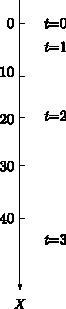
\includegraphics{figure/fig01.08}
    \\ ~ \\
    \caption{落体的运动}
    \label{fig:01.08}
\end{wrapfigure}
运动方程式、运动解。

为了便于进行计算,我们常希望能把轨迹
函数$x(t)$写成简单的分析表达式。对于表\ref{tab:01.04}~
的$x(t)$,可以写成
\begin{equation}\label{eqn:01.05.01}
    x=17t
\end{equation}
对于表\ref{tab:01.05}~的运动,可以写成$x=4.9t^2$。

对于曲线运动,轨迹函数就是位置矢量$\vec{r}$作为时间
$t$的函数,亦即$\vec{r}(t)$。随着$t$的变化,位置矢量$\vec{r}$的
端点在空间所划出的曲线,就是质点运动的轨迹(图\ref{fig:01.09})。也可
以用质点的三个坐标的函数$x(t)$,$y(t)$及$z(t)$来描写运
动,它们与$r(t)$的关系是
\clearpage
\begin{equation}\label{eqn:01.05.02}
    \vec{r}(t)=x(t)\vec{i}+y(t)\vec{j}+z(t)\vec{k}
\end{equation}

\begin{wrapfigure}[7]{r}{11em}
    \centering
    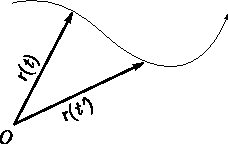
\includegraphics{figure/fig01.09}
    \caption{曲线运动}
    \label{fig:01.09}
\end{wrapfigure}
轨迹也具有相对性。譬如对于从地面上某一高度自由下落的质点,以
地面为参考系,看到轨迹是一条直线;而相对于沿平直铁轨稳定运行的
列车来说,轨迹则是一条抛物线。同一个物体的运动,在不同的参考系中
看到的轨迹形状不一定相同。

另一方面,对于时间,也必须选取一定的标准,即选取时间
原点,才能进行测量。而时间原点的选取,也有任意性,不同的
选取法,使轨迹函数的形式也有些差别。

因此,参考系的概念要作些扩充。选取一个参考系应包括:
给定放置在某物体上的坐标系,作为测量空间的标准;以及给定
一个钟,作为测量时间的标准。